This section describes the detailed implementation of SONIC in \CMSSW and the server technology used, the Triton Inference Server~\cite{triton} developed by NVIDIA. also discusses about the benefits of running inference with SONIC.

\subsection{Implementation in \CMSSW}

SONIC is implemented in \CMSSW through the ExternalWork framework component and accesses coprocessor resources on remote servers via gRPC calls, which is a cross-platform open source high performance Remote Procedure Call (RPC) framework originall developed by \Google~\cite{gRPC}. An illustration of this procedure, where client jobs make asynchronous, non-blocking gRPC calls to remote servers, is shown in Fig.~\ref{fig:architecture}. Multiple servers can run on multiple coprocessors, with load balancers in between. An important aspect of this scheme is that the client-side code does not need to be able to run any particular inference packages or frameworks; it simply has to collect the relevant input data for a trained model, communicate that information to the server in the expected format, and handle the output from the server.

\begin{figure}[htp]
    \centering
    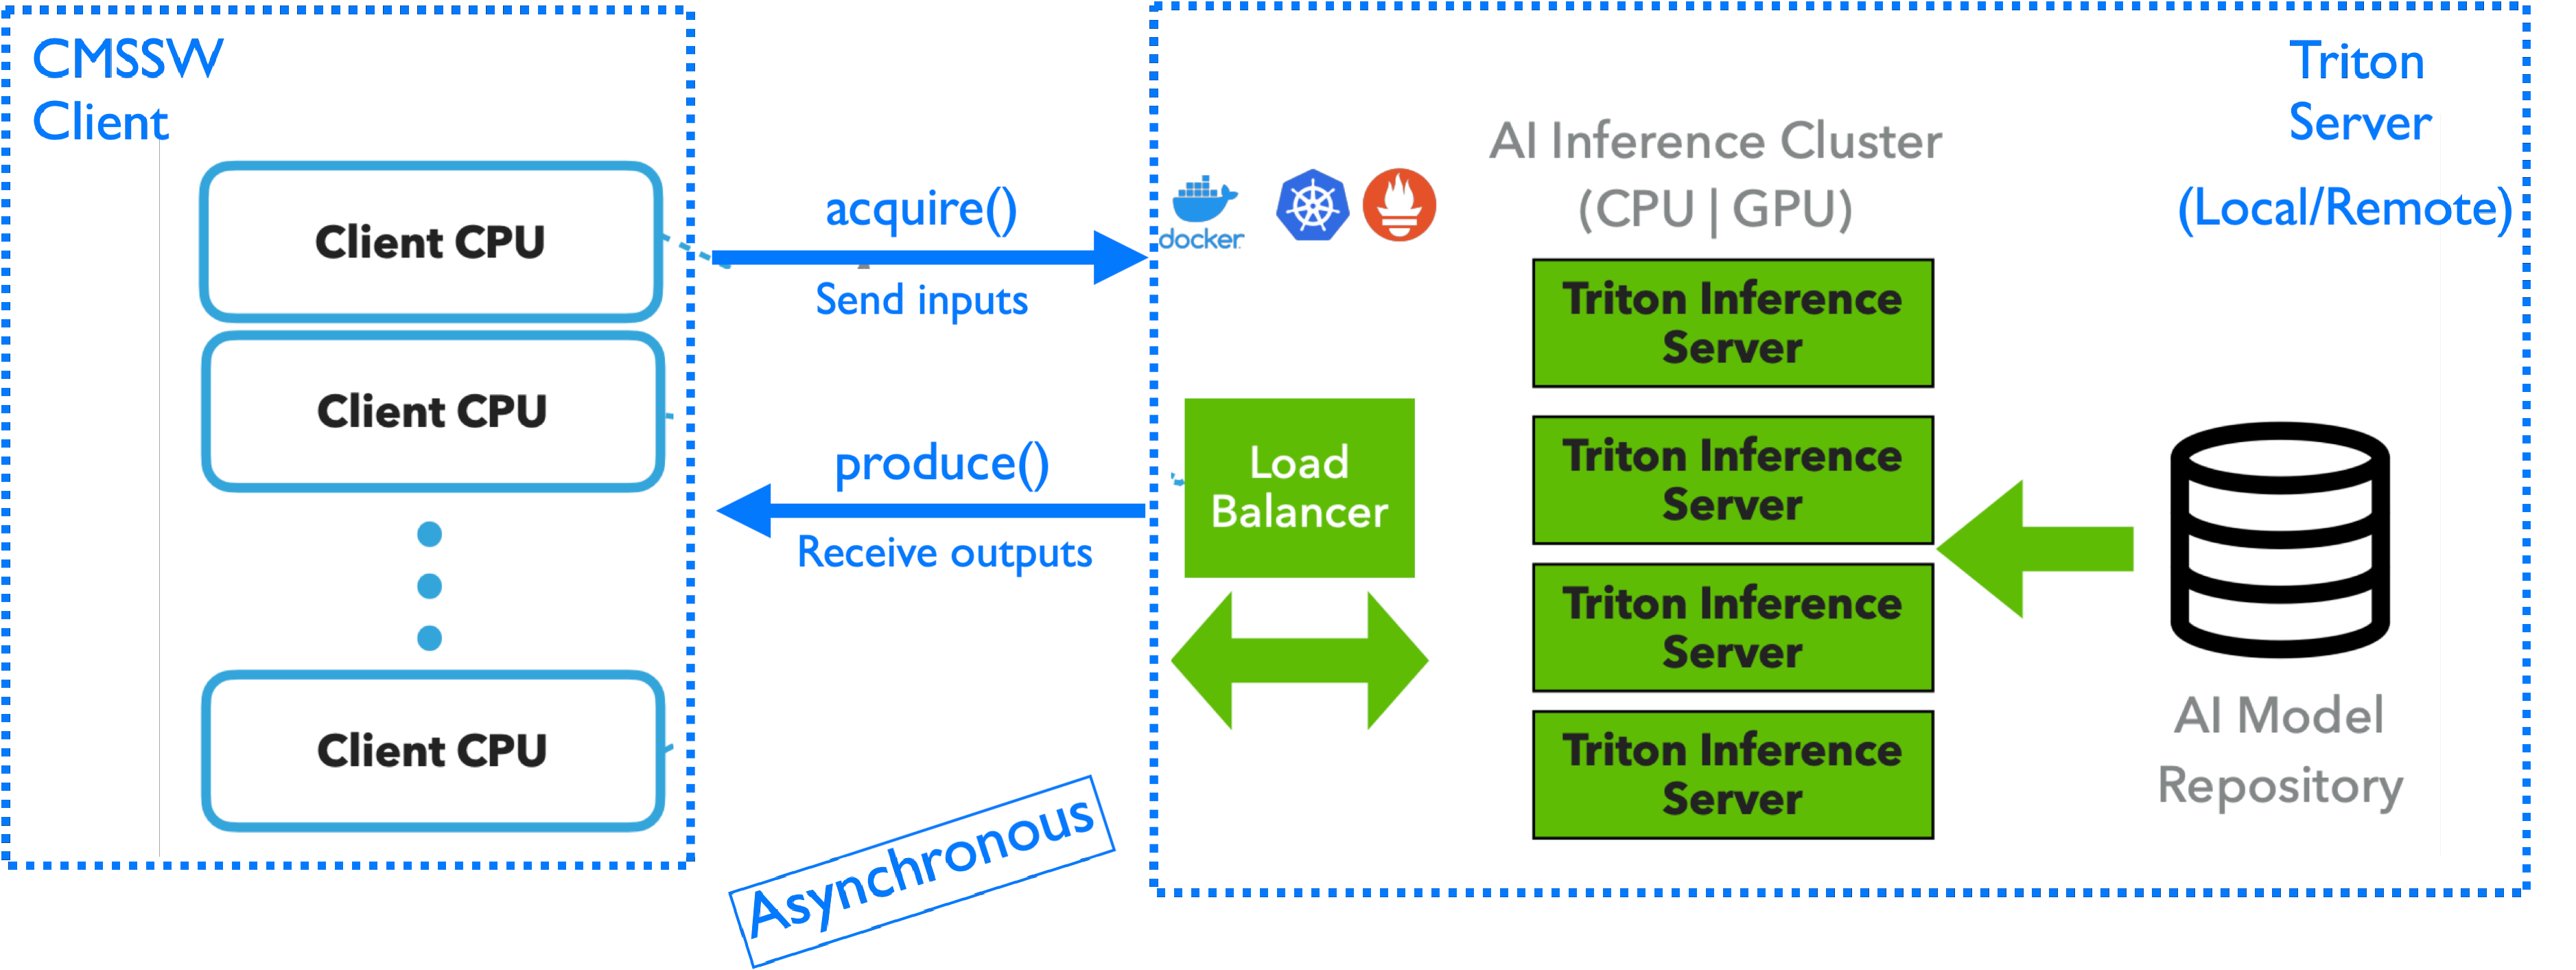
\includegraphics[width=0.90\textwidth]{plots/architecture.pdf}
    \caption{Illustration of the SONIC implementation of inference as-a-service in \CMSSW. This figure also shows the possibility of an additional load-balancing layer in the SONIC scheme; for example, if multiple coprocessor-enabled machines are used to host servers, a Kubernetes engine can be set up to distribute inference calls across the machines.}
    \label{fig:architecture}
\end{figure}

The client-side framework code for SONIC is split into two packages: a ``core'' package~\cite{SONIC_cms} containing class templates and other common infrastructure for the IaaS approach, and a dedicated package~\cite{SONIC_cms_triton} to interact specifically with the Triton server. SONIC modules provide a similar interface to standard \CMSSW modules. The partitioning into two packages reflects that the SONIC approach can be implemented for multiple server backends. For example, the first implementation~\cite{SONIC_origin,Duarte:2019fta} actually used the Microsoft Brainwave service~\cite{Brainwave}, which provides FPGA resources. In practice, given the generality and openness of the protocols used by Triton, which are themselves an extension of the KServe standard~\cite{KServe}, we expect that future development of SONIC will continue to use these protocols even if the backends or coprocessors change. Further discussion of different backends and coprocessors can be found in Section~\ref{sec:IPUs}.

Within CMSSW, a mechanism has been implemented to account for the possibility that a client job cannot access a specified server for whatever reason. In this case, a ``fallback'' server is automatically created using either GPU resources if they are available or the CPU resources allocated to the client job in question. The client then makes gRPC calls to that local fallback server, which introduces negligible latency. The server overhead generally consumes very little of the CPU resources beyond what would be used for conventional inference, such that the per-event latency is not strongly affected by SONIC relative to running without SONIC. Fallback servers are automatically shut down when the job finishes. Detailed studies related to these fallback servers are discussed later in Section~\ref{sec:fallback}.

\subsection{NVIDIA Triton Inference Server}
\label{sec:triton}
%Document a brief introduction about the NVIDIA Triton inference server
As shown in Fig.~\ref{fig:architecture}, currently the server-side implementation of SONIC in \CMSSW uses the NVIDIA Triton Inference Server for inference on coprocessors~\cite{triton, triton_readme}. Triton is an open-source solution whose protocols are public and extensible, as noted above. It supports inference of ML algorithms, or ``models'', in most modern formats, such as \PYTORCH, TensorRT, ONNX Runtime, \TENSORFLOW, and \XGBOOST. It also supports custom backends for alternative tasks, such as classical rule-based domain algorithms and inference on different types of coprocessors. Several features of Triton are worth highlighting:

\begin{itemize}
 \item \emph{Multiple model instances}: A single server can host multiple models at the same time or even multiple instances of the same model to allow concurrent inference requests.
 \item \emph{Dynamic batching}: Usually coprocessors have large number of processing units and the number of elements from one inference call is not enough to fully utilize coprocessors. With dynamic batching, if multiple inference calls are made within a window of time, the server can concatenate all calls' inputs into a single batch, which improves the GPU utilization and therefore increases the overall throughput.
 \item \emph{Model analyzer}: Parameters such as the number of model instances on a single server, the length of a batching window, and the optimal batch size are tunable and can be optimized on a case-by-case basis. Triton provides a model analyzer tool to aid in this optimization~\cite{triton_model_analyzer}. It can mimic the clients and send randomized inputs or some pre-saved data to the server. The server performance is measured and therefore the optimal deployment configuration can be determined by scanning the phase space.
 \item \emph{Ragged batching}: In HEP data, the number of inputs for inference can vary from one request to another, making it harder to batch them together. Ragged batching allows inference requests with different sizes to be batched together, therefore improving the performance. 
\end{itemize}

Triton servers can use one or multiple GPUs on the same machine with a built-in load balancer. Triton servers can also run purely on CPU resources when there are no GPU resources available. For other types of coprocessors, Triton servers can also be used with the help of custom backends. To start a server, it is only necessary to provide a trained model file and sometimes a configuration file specifying input and output variable names, shapes, types, and model versions. Client-side jobs are configured with server addresses and port numbers in order to carry out communications, and modules must provide input with the correct format for inference.

% It is also possible to use those protocols in alternative server implementations, as was done in the FPGAs-as-a-Service Toolkit~\cite{FaaST}.%not strictly necessary to use Triton's set of protocols; for example, server protocols were independently reimplemented for communication with inference servers in the FPGAs-as-a-Service Toolkit~\cite{FaaST}.

\subsection{SONIC Discussion}
\label{sec:sonic_benefits}

\iffalse
This work was then extended to study the use of GPUs as coprocessors for multiple LHC-specific applications in Ref.~\cite{Krupa:2020bwg}. There, SONIC was used to enable acceleration of three algorithms:
\begin{enumerate}
    \item A ResNet-50 based top quark jet tagger;
    \item Fast Calorimeter Learning (FACILE), which is a deep neural network for CMS hadron calorimeter (HCAL) energy regression;
    \item DeepCalo, which is a convolutional neural network for electron and photon energy regression in the ATLAS electromagnetic calorimeter~\cite{deepcalo}.
\end{enumerate}
These algorithms represent a wide range of algorithmic complexity and input data size, and all of them show significant speed improvements when running via SONIC. While these algorithms provided an interesting and useful testbed, currently they are not run by default in either the ATLAS or CMS data-processing workflows.
\fi

IaaS, as implemented in the SONIC approach, provides a number of useful advantages and benefits, which are summarized here.
Many of these features arise from the differences between the IaaS approach and the more traditional approach of HEP software frameworks to use only local computing resources.
\begin{itemize}
    \item \emph{Containerization}: SONIC factorizes ML frameworks out of the client software stack, i.e., \CMSSW, making it easier to support a wide variety of ML models. Currently, all ML algorithms in \CMSSW must be implemented in one of a limited number of supported frameworks (\TENSORFLOW, \ONNX, and \XGBOOST). With SONIC, one can use any framework supported by Triton, including custom backends, without needing to modify the \CMSSW software stack to resolve library dependencies and ensure compatibility between all external packages. This allows physicists to pick the best ML training and inference backends with less concern for the implementation details.
    \item \emph{Simplicity}: Because of the containerization discussed above, SONIC client-side code is simpler and more general than the corresponding direct inference code. SONIC modules need only implement the conversion of input data into the server's desired format and the reverse operation for output data.
    \item \emph{Flexibility}: In the SONIC paradigm, the connections between client CPUs and server coprocessors are not fixed. The servers can be physically local or remote with respect to the clients. Clients from many different machines can access a single server running on either one coprocessor or multiple coprocessors. Similarly, a single client can access multiple different servers running on multiple different machines. 
    \item \emph{Efficiency}: SONIC enables balanced utilization of coprocessor resources. By optimizing the coprocessor-to-CPU ratio for different tasks, it is easier to saturate coprocessor resources without oversaturating them. Because of this, any GPU purchase can be kept to the minimal number of GPUs necessary, saving overall cost.
    \item \emph{Portability}: Through the use of SONIC, client-side code does not have to be modified to take advantage of different types of coprocessors. Only a consistent protocol for communicating with the inference server is required, regardless of the underlying hardware: CPU, GPU, FPGA, IPU, or any other architecture.
    \item \emph{Accessibility}: If GPUs or other coprocessors are not available locally, the only way to accelerate workflows is to access those resources remotely, as a service. SONIC implements this use case for CMS. In addition to the other benefits listed above, remote access allows collaborators to share resources more easily. While calls to a remote server introduce a distance-dependent latency, the use of asynchronous calls in SONIC means that the overall event latency is negligibly impacted~\cite{Krupa:2020bwg}. SONIC can also use local resources if they are available.
\end{itemize}

However, with these advantages come additional complexity and changes in resource usage.
Production jobs using SONIC will rely on a separate server running separate software, compared to the existing scheme in which jobs only execute \CMSSW on local hardware.
\begin{itemize}
\item \emph{Server failures}: inference servers, remote or local, may experience software or hardware failures that prevent them from continuing to run. These new failure modes are mostly uncorrelated with existing known sources of failures, potentially leading to an overall increase in the rate of job failures. However, these failures can be mitigated with both server-side technology such as Kubernetes and client-side protocols such as the local fallback server.
\item \emph{Network usage}: the use of remote inference servers necessarily implies an increase in network traffic, as input and output data must be communicated over the network. Typically, input data are much larger than output data; the total usage depends on the algorithm. For the mini-AOD production workflow tests presented here, the network usage is discussed in Section~\ref{sec:scale_out}. High network usage can be mitigated using compression, with some tradeoff in throughput from the additional operations to compress and decompress the data.
\item \emph{Memory usage}: the use of remote inference servers actually reduces the local memory usage of production jobs, compared to the direct inference approach. However, the use of local fallback servers, whether to mitigate remote server failures or to take advantage of SONIC's containerization and portability features, implies increased memory usage. Running the server process locally is generally expected to use more memory than the corresponding direct inference libraries. Measurements of memory usage are presented in Section~\ref{sec:fallback}.
\end{itemize}
These potential drawbacks, especially uncorrelated failures and network usage, are similar to those from other distributed services used in CMS production, such as the conditions database or XRootD~\cite{Guida:2015gvw,Bauerdick:2012st}.
In practice, these additional failures and resource usage are usually found to be small enough that they do not outweigh the benefits of using distributed services.